\documentclass[aspectratio=169,11pt]{beamer}
\usepackage{teaching_slides}
\usepackage{listings}

\lstset{
  language=R,
  basicstyle=\ttfamily\tiny,
  backgroundcolor=\color{gray!5},
  frame=single,
  rulecolor=\color{gray!50},
  keywordstyle=\color{blue!70!black},
  commentstyle=\color{green!40!black},
  stringstyle=\color{orange!90!black},
  columns=flexible,
  keepspaces=true,
  showstringspaces=false,
  breaklines=true
}

\usepackage{inconsolata} % nice monospace font

\title[L10 - RDD]{ Econometrics I}
\subtitle{Lecture 10: Regression Discontinuity}
\author{Chris Conlon \\NYU Stern}
\date{Fall 2026}

% Rebuilt November 2026. Simulation-first: the running example is the Session 9 SOX-404 mandate,
% now as a cross-section at the $75M public-float threshold (Iliev 2010), with known truth.
% Float management (Gao, Wu and Zimmerman 2009) is the manipulation case; Burgstahler-Dichev the
% field bunching example. Readings: Goff Ch. 5; Mixtape (Remix) Ch. 6; Cattaneo, Idrobo and
% Titiunik, "A Practical Introduction to Regression Discontinuity Designs: Foundations".
% Figures/tables: rdd_sims.R. Workbook: inclass_session10.Rmd.

\begin{document}
\frame{\titlepage}


\begin{frame}{Where we are}
\begin{itemize}
	\item Session 9: SOX Section 404 hit firms with public float of at least \$75M and exempted smaller ones.
	DiD compared the two groups over time and needed parallel trends.
	\medskip
	\item The DiD slides ended on a warning: treatment is assigned \emph{by} size, so treated and exempt firms
	overlap only near \$75M.
	\medskip
	\item Today: make that the design. Compare firms just above \$75M to firms just below it, in one year.
	\begin{itemize}
		\item What it identifies, and the one assumption that buys it.
		\item How to estimate a jump at a point without trusting a functional form.
		\item How it breaks (firms manage their float) and how to tell.
		\item What to do when the cutoff only shifts the \emph{probability} of treatment.
	\end{itemize}
	\medskip
	\item Simulated throughout, so we always know the right answer.
\end{itemize}
\end{frame}


\begin{frame}{How do we construct the counterfactual?}
We observe $Y_i(D_i)$ but never $Y_i(1-D_i)$. Ways to fill in the missing cell:
\begin{description}
	\item [Matching:] a unit $j$ with $X_j = X_i$ but $D_j \ne D_i$. Needs overlap: both treated and untreated
	units at each $X$.
	\item [Difference-in-differences:] the \emph{change} in other units. Needs parallel trends.
	\item [\alert{Regression discontinuity:}] treatment is a deterministic function of $X$, so overlap fails
	everywhere. Instead, compare units just on either side of the cutoff, where they should be alike in
	everything except treatment.
	\item [Instrumental variables:] a shifter of treatment that affects $Y$ only through $D$. A fuzzy RD is
	exactly this, with the cutoff as the instrument.
\end{description}
\end{frame}


\section{The design}

\begin{frame}{Setup}
\begin{itemize}
	\item A \alert{running variable} $X_i$ (also: forcing variable, score) and a known \alert{cutoff} $c$.
	\medskip
	\item \alert{Sharp} design: treatment is a deterministic function of the score,
	\[
		D_i = \mathbf{1}\{X_i \ge c\}.
	\]
	\item \alert{Fuzzy} design: the \emph{probability} of treatment jumps at $c$, but not from 0 to 1.
	\medskip
	\item Examples: a regulation that applies above a size threshold; a credit score below which loans are
	not securitized; an index that holds the 1,000 largest stocks; a badge awarded above a rating.
	\medskip
	\item The design problem: at any given $x$, every unit is treated or every unit is untreated. There is no
	$x$ at which we see both. Matching on $X$ is impossible, by construction.
\end{itemize}
\end{frame}


\begin{frame}{Identification: continuity}
\begin{itemize}
	\item Assume $\E[Y_i(0) \mid X_i = x]$ and $\E[Y_i(1) \mid X_i = x]$ are \alert{continuous} in $x$ at $c$.
	\item In a sharp design, $\E[Y_i \mid X_i = x] = \E[Y_i(1) \mid X_i = x]$ for $x \ge c$ and
	$\E[Y_i(0) \mid X_i = x]$ for $x < c$. Take limits from each side:
	\[
		\tau_{SRD} \equiv \lim_{x \downarrow c} \E[Y_i \mid X_i = x] - \lim_{x \uparrow c} \E[Y_i \mid X_i = x]
		= \E[Y_i(1) - Y_i(0) \mid X_i = c].
	\]
	(Hahn, Todd and van der Klaauw 2001.)
	\medskip
	\item What this buys: the average effect \alert{for units at the cutoff}. Nothing about firms with \$500M of
	float without more assumptions.
	\medskip
	\item What it costs: continuity is about potential outcomes, so it cannot be tested directly. It fails if
	something else also changes at $c$, or if units can choose which side of $c$ they land on.
\end{itemize}
\end{frame}


\begin{frame}{Running example: SOX Section 404 at \$75M}
\begin{itemize}
	\item Accelerated filers (public float $\ge$ \$75M) needed an auditor attestation of internal controls from
	fiscal 2004; smaller firms were exempt. Iliev (2010, \emph{JF}) uses exactly this threshold.
	\medskip
	\item \alert{Our simulation:} 4,000 firms in fiscal 2004.
	\begin{itemize}
		\item Running variable $x = \log(\text{float} / \$75\text{M})$, so the cutoff is $x = 0$. Same float
		distribution as Session 9.
		\item Outcome: log audit fee. Bigger firms pay more, along a smooth, \emph{curved} function of $x$.
		\item True jump at the cutoff: $\tau = 0.35$, the same first-year effect as in Session 9.
		\item We also record fiscal 2002 audit fees, before SOX existed.
	\end{itemize}
	\medskip
	\item Note what changed from DiD: one year, no pre-period needed for identification. The comparison is
	across firms at nearly the same size.
\end{itemize}
\end{frame}


\begin{frame}{The picture}
\begin{center}
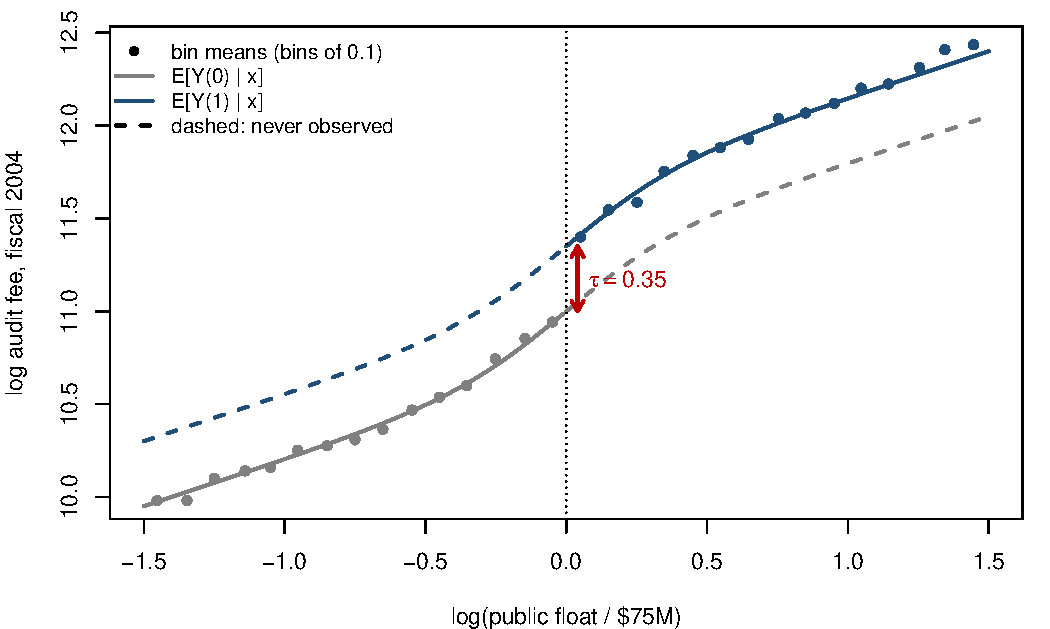
\includegraphics[height=0.82\textheight]{fig_rd_sharp.pdf}
\end{center}
\end{frame}


\begin{frame}{Why should we believe continuity?}
\begin{itemize}
	\item Lee (2008): if units have only \alert{imprecise control} over $X$, the luck component near $c$ makes
	treatment \emph{as good as randomly assigned} in a small neighborhood of $c$.
	\begin{itemize}
		\item A firm can aim for more or less float, but its share price on the measurement date is noisy.
		\item The classic case: close elections. Barely winning and barely losing candidates are alike.
	\end{itemize}
	\medskip
	\item This turns an untestable assumption into testable predictions, as in a randomized experiment:
	\begin{enumerate}
		\item The \alert{density} of $X$ is smooth at $c$. No pile-up on the favorable side.
		\item \alert{Pre-treatment covariates} do not jump at $c$. (Here: fiscal 2002 audit fees.)
	\end{enumerate}
	\medskip
	\item If agents have \alert{precise} control over $X$ and care about treatment, both predictions fail. We
	will make that happen below.
\end{itemize}
\end{frame}


\section{Estimation}

\begin{frame}{Estimation is extrapolation to a boundary}
\begin{itemize}
	\item We need two limits: $\E[Y \mid X = c]$ approached from the right, and from the left. There are no
	data \emph{at} $c$ from either side; each side's value at $c$ is an extrapolation to the edge of its data.
	\medskip
	\item Two families of estimators:
	\begin{itemize}
		\item \alert{Global}: fit a polynomial in $x$ on each side using all the data, evaluate at $c$.
		\item \alert{Local}: fit a line on each side using only data within $h$ of $c$, weighted toward $c$.
	\end{itemize}
	\medskip
	\item A kernel average (Nadaraya--Watson) is the worst choice here: at a boundary it averages points that
	all lie on one side, so it is biased whenever $\E[Y \mid X]$ has a slope. Fitting a line removes that bias.
	\medskip
	\item Either way, include the score on each side \emph{separately}: $y$ on $D$, $x - c$, and $D \times (x - c)$.
	The coefficient on $D$ is the jump at $c$.
\end{itemize}
\end{frame}


\begin{frame}{The same data, eight estimators}
\begin{center}
\small
\begin{tabular}{lccc}\toprule
Specification & Estimate & 95\% CI & Obs.\ used \\ \midrule
Global polynomial, order 1 each side & 0.692 & [0.66, 0.73] & 4,000 \\
Global polynomial, order 2 each side & 0.531 & [0.49, 0.58] & 4,000 \\
Global polynomial, order 3 each side & 0.414 & [0.36, 0.47] & 4,000 \\
Global polynomial, order 4 each side & 0.337 & [0.27, 0.40] & 4,000 \\
Global polynomial, order 5 each side & 0.325 & [0.25, 0.40] & 4,000 \\
\midrule
Local linear, triangular, $h = 0.47$ (by hand, \texttt{feols}) & 0.357 & [0.28, 0.43] & 1,211 \\
\texttt{rdrobust}: bias-corrected, robust CI & 0.339 & [0.25, 0.42] & 1,211 \\
\midrule
Truth & 0.350 & &  \\
\bottomrule\end{tabular}

\end{center}
\small
\begin{itemize}
	\item A global line mistakes curvature for a jump: $0.69$ against $0.35$, with a tight CI. Higher orders
	move toward the truth, but which order would you have reported without knowing it?
	\item Local linear uses the 1,211 firms within $h$ of the cutoff and lands close.
\end{itemize}
\end{frame}


\begin{frame}{Why not global polynomials (Gelman and Imbens 2019)}
\begin{center}
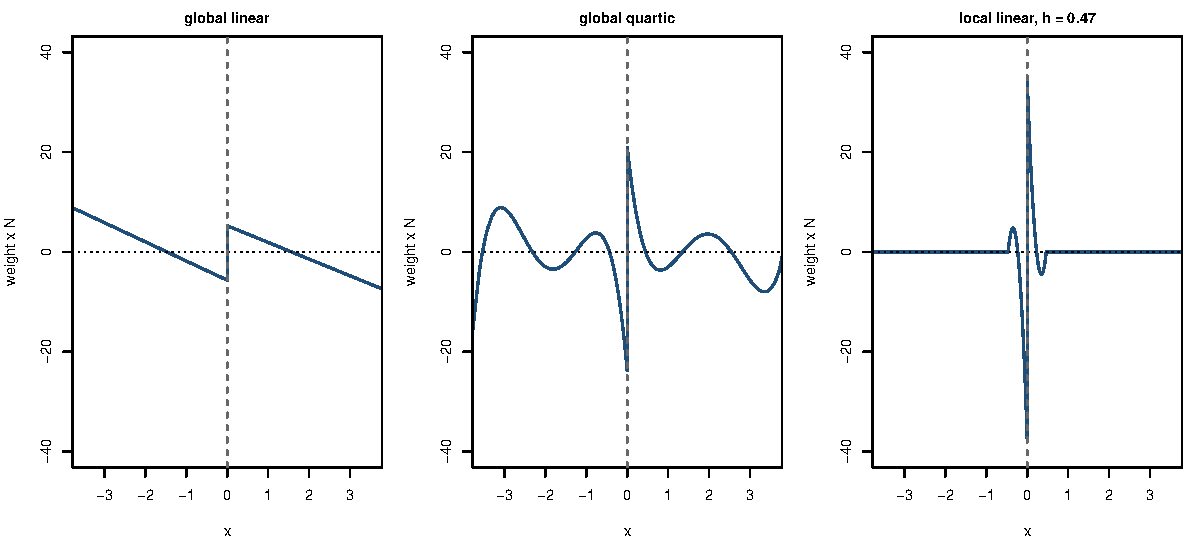
\includegraphics[height=0.5\textheight]{fig_rd_weights.pdf}
\end{center}
\small
Every estimator here is linear in $y$: $\hat\tau = \sum_i \omega_i y_i$. Plotted: $N \omega_i$ against $x_i$.
\begin{itemize}
	\item Global fits give large, sign-switching weights to firms far from \$75M: a firm with \$1.5B of float
	($x = 3$) moves the estimated jump at \$75M.
	\item Results are sensitive to the order, and conventional CIs undercover (next slides). Use local linear.
\end{itemize}
\end{frame}


\begin{frame}{Local linear regression}
For bandwidth $h$ and kernel $K$, solve
\[
	\min_{\alpha, \beta, \tau, \gamma} \sum_{i} K\!\left(\frac{x_i - c}{h}\right)
	\big(y_i - \alpha - \beta (x_i - c) - \tau D_i - \gamma D_i (x_i - c)\big)^2 .
\]
\begin{itemize}
	\item Triangular kernel $K(u) = (1 - |u|)\,\mathbf{1}\{|u| < 1\}$: weight falls linearly to zero at $h$.
	\item It is just weighted least squares on the subsample $|x_i - c| < h$: \texttt{feols} with \texttt{weights}.
	\medskip
	\item \alert{Bias--variance tradeoff} in $h$:
	\begin{itemize}
		\item Bias: the line misses the curvature. Roughly $\propto h^2 \times$ (second derivative of $\E[Y \mid X]$).
		\item Variance: fewer observations. Roughly $\propto 1/(N h)$.
	\end{itemize}
	\item Minimizing MSE gives $h_{MSE} \propto N^{-1/5}$ (Imbens and Kalyanaraman 2012; Calonico, Cattaneo and
	Titiunik 2014). In our data, $h_{MSE} = 0.47$: float between about \$47M and \$120M.
\end{itemize}
\end{frame}


\begin{frame}{The bandwidth tradeoff, against the truth}
\begin{center}
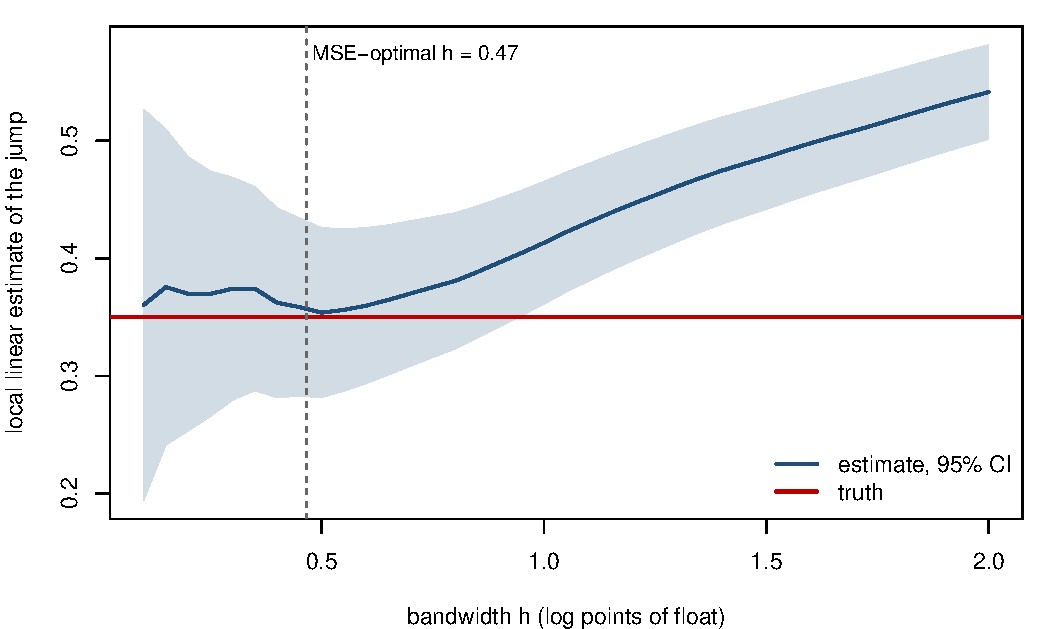
\includegraphics[height=0.72\textheight]{fig_rd_bandwidth.pdf}
\end{center}
\small Wider windows give tighter intervals around the wrong number: the curvature in audit fees leaks into the jump.
\end{frame}


\begin{frame}{The inference problem at $h_{MSE}$}
\begin{itemize}
	\item $h_{MSE}$ balances squared bias against variance, so at $h_{MSE}$ the bias is the \emph{same order} as
	the standard error. The conventional CI, $\hat\tau \pm 1.96\,\widehat{se}$, is centered in the wrong place.
	\medskip
	\item Fixes:
	\begin{itemize}
		\item \alert{Undersmooth}: use a smaller $h$ for inference. Valid, but there is no good rule for how small.
		\item \alert{Robust bias correction} (Calonico, Cattaneo and Titiunik 2014): estimate the bias with a
		local quadratic, subtract it, and widen the SE to account for the noise in the bias estimate. This is
		\texttt{rdrobust}'s default.
		\item Bias-aware ``honest'' intervals bound the curvature directly (Armstrong and Kolesár 2020).
	\end{itemize}
	\medskip
	\item Report: the conventional point estimate at $h_{MSE}$ (or the bias-corrected one) with the
	\alert{robust} CI.
\end{itemize}
\end{frame}


\begin{frame}{Monte Carlo: 500 draws of the SOX design}
\begin{center}
\small
\begin{tabular}{lcccc}\toprule
Estimator and CI & Bias & Std.\ dev. & Coverage of 95\% CI & CI length \\ \midrule
Global quartic, robust SE & 0.041 & 0.032 & 0.78 & 0.135 \\
Local linear at $h_{MSE}$, conventional CI & 0.020 & 0.042 & 0.91 & 0.161 \\
Local linear at $h_{MSE}$, robust bias-corrected CI & 0.020 & 0.042 & 0.96 & 0.174 \\
\bottomrule\end{tabular}

\end{center}
\medskip
\begin{itemize}
	\item The global quartic looked fine in our one draw. Across draws it is biased and its 95\% CI covers 78\% of the time.
	\item Local linear at $h_{MSE}$ (mean $h = 0.45$) with a conventional CI covers 91\%.
	\item Same point estimate, robust bias-corrected CI: 96\%, for a CI about 8\% longer.
\end{itemize}
\end{frame}


\begin{frame}[fragile]{In practice}
\begin{lstlisting}
library(rdrobust)
rd <- rdrobust(d$y, d$x, c = 0)          # local linear, triangular kernel, h_MSE, robust bias-corrected CI
summary(rd)                               # report "Conventional" coef with the "Robust" CI
rdplot(d$y, d$x, c = 0)                   # binned means + global fits: a picture, not an estimator
rdbwselect(d$y, d$x, c = 0)               # bandwidths only

h <- rd$bws["h", "left"]                  # the same estimate by hand
s <- subset(d, abs(x) < h); s$k <- 1 - abs(s$x) / h
feols(y ~ D * x, s, weights = ~k, vcov = "hetero")   # coefficient on D = rdrobust's conventional estimate
\end{lstlisting}
\begin{lstlisting}[language=Python]
from rdrobust import rdrobust, rdplot     # pip install rdrobust rddensity
rd = rdrobust(y=d.y, x=d.x, c=0); print(rd)
\end{lstlisting}
\begin{itemize}
	\item Center the score at the cutoff. Interact everything with $D$.
	\item Show sensitivity: half and double $h_{MSE}$, and a different kernel. The estimate should not swing.
\end{itemize}
\end{frame}


\begin{frame}{Pictures: binscatter done right}
\begin{center}
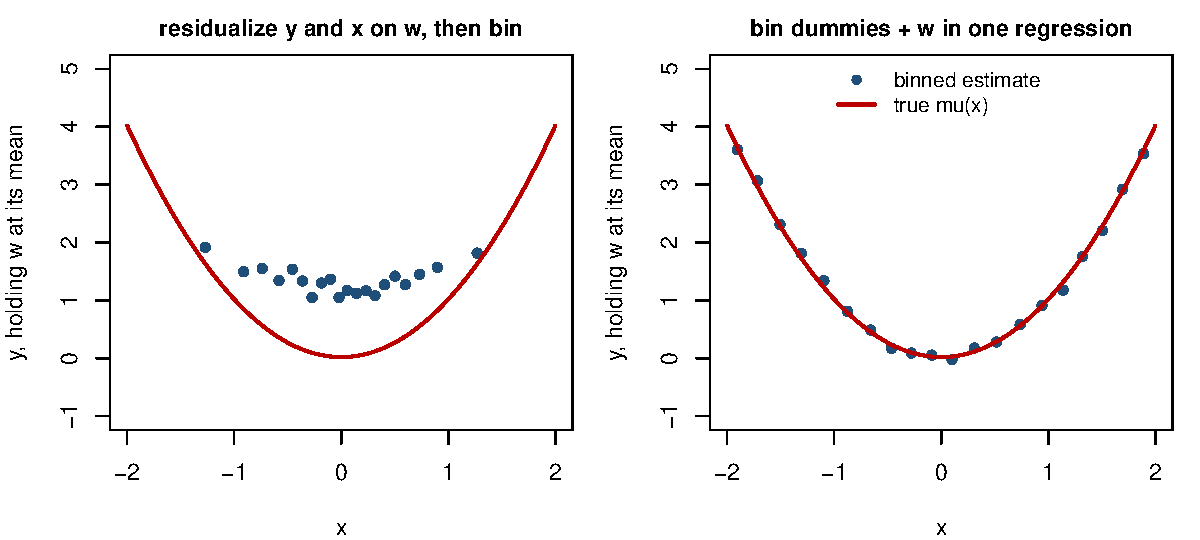
\includegraphics[height=0.52\textheight]{fig_rd_binscatter.pdf}
\end{center}
\small
\begin{itemize}
	\item Every RD paper shows binned means. With covariates $w$, the common shortcut (residualize $y$ and $x$ on
	$w$, then bin) distorts the shape of $\E[y \mid x]$: the truth here is $x^2$.
	\item Instead, regress $y$ on bin dummies and $w$ together (Cattaneo, Crump, Farrell and Feng 2024, \emph{AER}).
	\texttt{binsreg} in R, Stata, and Python.
\end{itemize}
\end{frame}


\section{Is the design valid?}

\begin{frame}{The main threat: firms choosing their side}
\begin{itemize}
	\item Gao, Wu and Zimmerman (2009, \emph{JAR}): after SOX, firms near \$75M kept their public float under the
	threshold. They invested less, paid out more cash, and reduced shares held by non-affiliates.
	\medskip
	\item \alert{Our simulation:} firms with true float between \$75M and \$96M, and \emph{high} audit costs,
	push reported float just under \$75M. 147 of the 344 eligible firms do it.
	\medskip
	\item They stay exempt but keep the audit fees of their true size and costs. Two problems at once:
	\begin{itemize}
		\item Just below \$75M, the exempt group now includes bigger, costlier firms.
		\item Just above, the remaining accelerated filers are the low-cost ones.
	\end{itemize}
	Both push the estimated jump down.
\end{itemize}
\end{frame}


\begin{frame}{Symptom 1: the density of the running variable}
\begin{center}
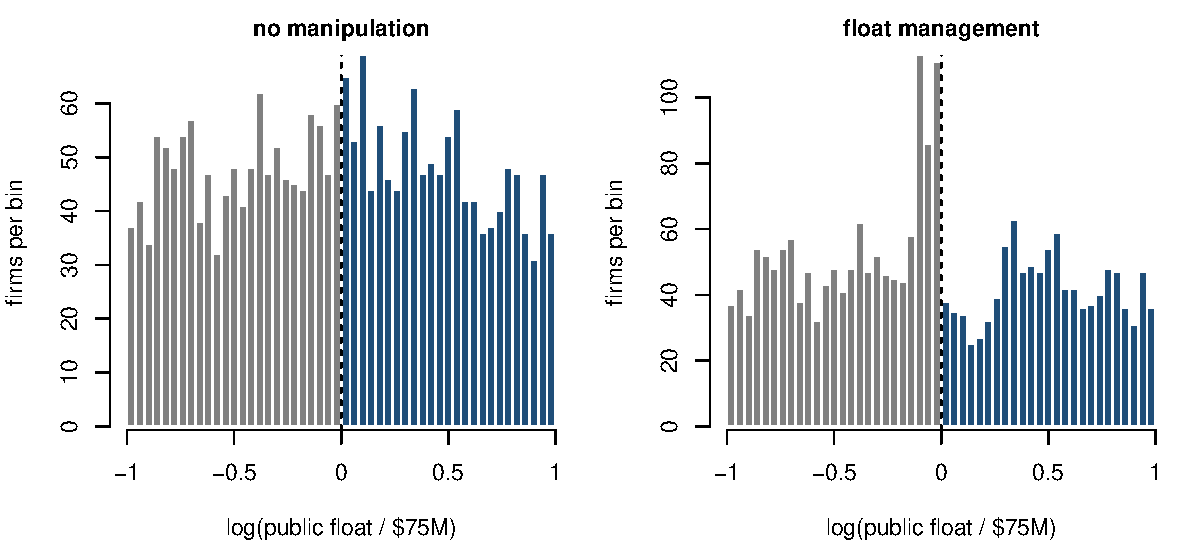
\includegraphics[height=0.66\textheight]{fig_rd_density.pdf}
\end{center}
\small McCrary (2008); Cattaneo, Jansson and Ma (2020, \emph{JASA}): estimate the density of $x$ on each side
with local polynomials and test for a jump. \texttt{rddensity} in R, Stata and Python.
\end{frame}


\begin{frame}{Symptom 2: pre-treatment variables jump. And the donut}
\begin{center}
\small
\resizebox{\textwidth}{!}{\begin{tabular}{lccc}\toprule
Sample & Jump in 2004 fees (truth 0.35) & Jump in 2002 fees (truth 0) & Density test $p$ \\ \midrule
No manipulation & 0.339 [0.25, 0.42] & 0.013 [-0.07, 0.10] & 0.800 \\
Float management & 0.022 [-0.06, 0.11] & -0.292 [-0.39, -0.20] & 0.000 \\
Float management, donut $|x| < 0.15$ dropped & 0.074 [-0.26, 0.41] & -0.120 [-0.40, 0.16] & --- \\
Float management, donut $|x| < 0.30$ dropped & 0.515 [0.23, 0.80] & 0.165 [-0.11, 0.44] & --- \\
\bottomrule\end{tabular}
}
\end{center}
\small
\begin{itemize}
	\item With float management, the 2004 jump collapses to zero. Both diagnostics fire: the density test rejects,
	and \emph{2002} audit fees, set before SOX existed, ``jump'' by $-0.29$ at \$75M.
	\item A \alert{donut} RD drops firms near the cutoff, where the manipulators are. It removes them, but then
	extrapolates across the hole. With a curved $\E[Y \mid X]$, the estimate is noisy and biased (note the 2002 placebo).
	\item There is no estimator that repairs manipulation. The diagnostics tell you not to trust the design.
\end{itemize}
\end{frame}


\begin{frame}{Bunching in the field: earnings at zero}
\begin{columns}[T]
\begin{column}{0.55\textwidth}
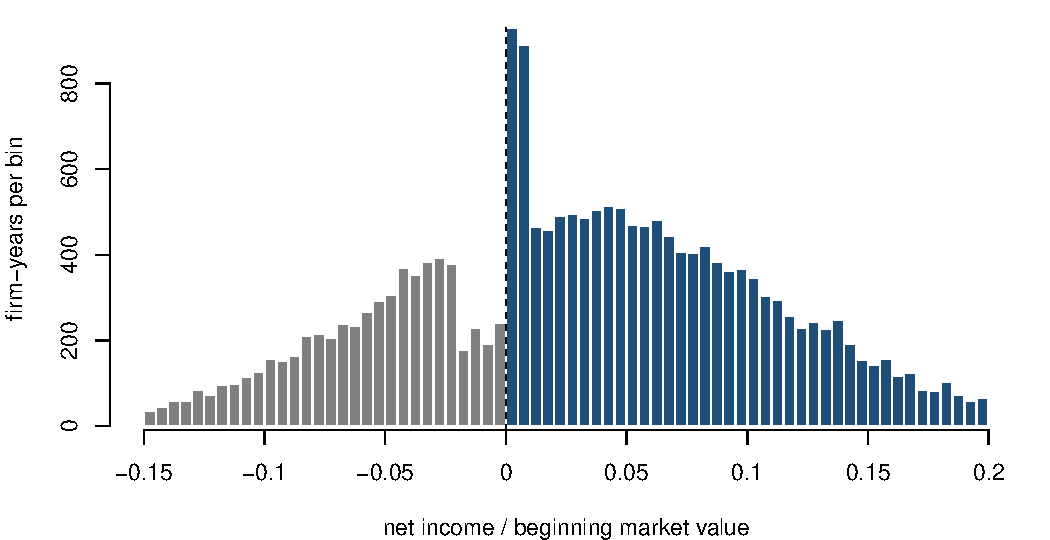
\includegraphics[width=0.95\textwidth]{fig_rd_bd.pdf}
\end{column}
\begin{column}{0.43\textwidth}
\small
\begin{itemize}
	\item Burgstahler and Dichev (1997, \emph{JAE}): too few firms report small losses and too many report small
	profits. Read as earnings management to avoid a loss.
	\item Simulated here: half of firms with small losses report a small profit instead. Density test
	$p$ = $<0.001$
.
	\item Caution: Durtschi and Easton (2005, \emph{JAR}) show scaling and sample selection can also bend
	these histograms near zero.
	\item For RD, the lesson is the same: any threshold that matters to the agent is a reason to check the density.
\end{itemize}
\end{column}
\end{columns}
\end{frame}


\begin{frame}{More checks}
\begin{itemize}
	\item \alert{Placebo cutoffs}: estimate a ``jump'' at points where nothing happens, using data on one side
	only. You should find nothing.
	\medskip
	\item \alert{Placebo outcomes}: covariates and lagged outcomes, as above.
	\medskip
	\item \alert{Bandwidth and kernel sensitivity}: half and double $h_{MSE}$; uniform vs.\ triangular.
	\medskip
	\item \alert{Compound treatments}: does anything else change at the same cutoff? The \$75M line also defined
	accelerated filers for other SEC rules, including earlier 10-K deadlines. RD estimates the effect of
	\emph{everything} that switches at $c$.
	\medskip
	\item \alert{Do not} add covariates to fix imbalance. Covariates can tighten the CI in a valid design; they
	cannot rescue an invalid one.
\end{itemize}
\end{frame}


\section{Fuzzy RD}

\begin{frame}{When the cutoff shifts the probability of treatment}
\begin{itemize}
	\item Some exempt firms obtain the attestation voluntarily; some accelerated filers get extensions or miss it.
	The cutoff changes $\Pr(D = 1 \mid X)$ but not from 0 to 1.
	\[
		\tau_{FRD} = \frac{\lim_{x \downarrow c} \E[Y \mid X = x] - \lim_{x \uparrow c} \E[Y \mid X = x]}
		{\lim_{x \downarrow c} \Pr(D = 1 \mid X = x) - \lim_{x \uparrow c} \Pr(D = 1 \mid X = x)}
	\]
	\item This is a Wald estimator with $Z = \mathbf{1}\{X \ge c\}$ as the instrument for $D$. With
	monotonicity it is a \alert{LATE}: the effect for \emph{compliers at the cutoff}, firms that attest
	because they crossed \$75M and would not have otherwise.
	\medskip
	\item Estimation: 2SLS within the bandwidth, with the score on each side as controls. Same kernel and $h$
	for the first stage and the reduced form.
	\medskip
	\item \alert{Our simulation:} low-cost firms are more likely to attest on either side. 18\% attest below the
	cutoff, 78\% above.
\end{itemize}
\end{frame}


\begin{frame}{First stage and reduced form}
\begin{center}
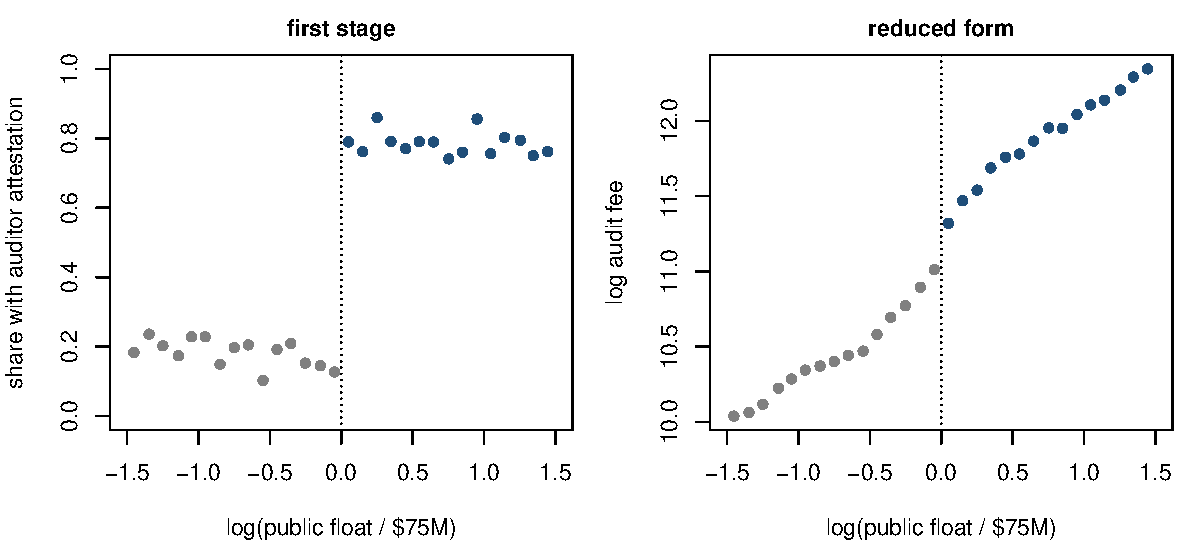
\includegraphics[height=0.66\textheight]{fig_rd_fuzzy.pdf}
\end{center}
\small The jump in audit fees is smaller than in the sharp design because only some firms switch status at \$75M.
Dividing by the jump in attestation rescales it to a per-attesting-firm effect.
\end{frame}


\begin{frame}{Fuzzy RD estimates}
\begin{center}
\small
\begin{tabular}{lcc}\toprule
Within $h = 0.80$, triangular kernel & Estimate & 95\% CI \\ \midrule
OLS: $y$ on compliance $D$ (and $x$ terms) & 0.111 & [0.08, 0.15] \\
First stage: jump in $\Pr(D \mid x)$ & 0.659 & [0.59, 0.73] \\
Reduced form: jump in $\E[y \mid x]$ & 0.250 & [0.19, 0.31] \\
Wald ratio = 2SLS with $Z = \mathbf{1}\{x \ge 0\}$ as instrument & 0.379 & [0.29, 0.47] \\
\texttt{rdrobust(..., fuzzy = D)}: bias-corrected, robust CI & 0.291 & [0.18, 0.40] \\
\midrule
Truth (every firm's effect) & 0.350 &  \\
\bottomrule\end{tabular}

\end{center}
\small
\begin{itemize}
	\item OLS on attestation is badly biased: firms that attest are low-cost firms.
	\item Reduced form $\div$ first stage $= 0.250 / 0.659 = 0.379$, exactly 2SLS, exactly \texttt{rdrobust}'s
	conventional fuzzy estimate. The robust CI from \texttt{rdrobust} covers the truth.
	\item The usual IV cautions apply: a weak first stage makes the ratio unstable.
\end{itemize}
\end{frame}


\section{Extensions}

\begin{frame}{Discrete scores, kinks, and other designs}
\begin{itemize}
	\item \alert{Discrete running variable} (test scores, ages in years, rounded ratings): there are no
	observations arbitrarily close to $c$, so ``local'' runs out. Kolesár and Rothe (2018, \emph{AER}): the
	common fix of clustering on the score makes things worse; use bounds on the curvature instead.
	\medskip
	\item \alert{Local randomization}: in a small window, treat assignment as random and use randomization
	inference (Cattaneo, Frandsen and Titiunik 2015). \texttt{rdlocrand}.
	\medskip
	\item \alert{Regression kink}: the \emph{slope} of a policy in $x$ changes at $c$ (tax brackets, benefit
	formulas). Estimate the change in slope of $\E[Y \mid X]$ divided by the change in slope of the policy
	(Card, Lee, Pei and Weber 2015, \emph{Econometrica}).
	\medskip
	\item \alert{Away from the cutoff}: the RD effect is local. Extrapolating needs extra structure, such as
	conditional independence given other covariates (Angrist and Rokkanen 2015, \emph{JASA}).
\end{itemize}
\end{frame}


\begin{frame}{RD in your fields}
\small
\begin{itemize}
	\item \alert{Accounting.}
	\begin{itemize}
		\item SOX 404 at \$75M: costs, earnings quality and stock prices (Iliev 2010, \emph{JF}).
		\item Firms keeping their float under \$75M (Gao, Wu and Zimmerman 2009, \emph{JAR}).
	\end{itemize}
	\item \alert{Finance.}
	\begin{itemize}
		\item Lenders screen less carefully just above the FICO 620 securitization rule of thumb (Keys,
		Mukherjee, Seru and Vig 2010, \emph{QJE}).
		\item Price effects of moving between the Russell 1000 and 2000 (Chang, Hong and Liskovich 2015, \emph{RFS}).
	\end{itemize}
	\item \alert{Marketing / IS.}
	\begin{itemize}
		\item Half-star rounding of Yelp ratings and restaurant reservations (Anderson and Magruder 2012, \emph{EJ}).
		\item The value of eBay's Top-Rated Seller badge (Elfenbein, Fisman and McManus 2015, \emph{AEJ: Micro}).
	\end{itemize}
	\item Reading one: find the score, the cutoff, who sets the cutoff, and whether the agents can move.
\end{itemize}
\end{frame}


\begin{frame}{Checklist}
\begin{enumerate}
	\item Plot $\Pr(D \mid X)$: sharp or fuzzy? How big is the first stage?
	\item Plot $\E[Y \mid X]$ with binned means. Is the jump visible?
	\item Density of $X$ at $c$ (\texttt{rddensity}), and the story for why agents could or could not sort.
	\item Covariates and lagged outcomes at $c$: no jumps.
	\item Main estimate: local linear, triangular kernel, $h_{MSE}$, robust bias-corrected CI (\texttt{rdrobust}).
	\item Sensitivity: bandwidths, kernels, donut. Placebo cutoffs.
	\item Fuzzy: report first stage, reduced form and the ratio.
	\item Say whose effect it is: units at the cutoff (compliers at the cutoff, if fuzzy).
\end{enumerate}
\end{frame}


\begin{frame}{Recap}
\begin{itemize}
	\item RD replaces overlap with continuity: units just on either side of a cutoff stand in for each other.
	\medskip
	\item The estimand is local, at the cutoff. Estimating it is extrapolation to a boundary from each side.
	\medskip
	\item Use local linear regression, not global polynomials. At the MSE-optimal bandwidth, use robust
	bias-corrected inference.
	\medskip
	\item The design fails when agents can choose their side. Check the density and pre-treatment variables;
	no estimator fixes sorting.
	\medskip
	\item Fuzzy RD is IV with the cutoff as instrument, and it estimates a LATE for compliers at the cutoff.
\end{itemize}
\end{frame}


\begin{frame}{Workbook time}
\texttt{Fall/L10 - More Quasi Experiments/inclass\_session10.Rmd}:
\begin{enumerate}
	\item Reproduce the sharp estimate by hand and with \texttt{rdrobust}. Then make the audit-fee curve
	straighter: what happens to the global linear estimate and to $h_{MSE}$?
	\item Shrink the sample to 1,000 firms and redo the Monte Carlo. Does robust bias correction still fix coverage?
	\item Turn on float management. Vary how strongly it selects on audit costs, and find where the density
	test and the 2002 placebo stop detecting it.
	\item Fuzzy: weaken the first stage until the 2SLS estimate becomes unstable.
\end{enumerate}
\end{frame}

\end{document}
